\documentclass{article}

\usepackage{amsmath}
\usepackage{booktabs}  % nice tables
\usepackage[margin=25mm]{geometry}
\usepackage{natbib}
\usepackage{siunitx}  % use for all units
\usepackage{subcaption}  % for subfigures
\usepackage{todonotes}

\def\kph{\kilo\meter\per\hour}
\def\mps{\meter\per\second}

\title{Bicycle Balance Assistance Reduces Probability of Falling at Low Speeds
When Subjected to Mechanical Perturbations}

\author{Marten T. Haitjema \and Leila Alizadehsaravi \and Jason K. Moore}

\begin{document}

\maketitle

\abstract{
  Uncontrolled bicycles are generally unstable at low speeds. We add a
  controlled steering motor to a consumer bicycle that stabilizes the bicycle
  at low speeds. To test the motor's assistance during falls, we apply varying
  magnitude external handlebar perturbations to the bicycle while ridden on a
  treadmill with the balance assist system activated and deactivated.  The
  probability of not recovering from a handlebar perturbation decreases when
  the balance assist is activated at a speed of 6~\si{\kph}.
}

\section{Introduction}
%
Single-actor bicycle crashes are associated with a surprisingly large number of
reported injuries~\citep{Wegman2024}. At low speeds, from start up to typical
cruising speeds, bicycles themselves are not self-stable and can be challenging
for the rider to balance. Low speed crashes may be reduced if the bicycle was
self-stable at these speeds by relieving the rider of a necessary control
activity. Bicycles can be mechanically modified to lower the speeds at which
they are self-stable~\citep{Astrom2005} and since the 1980s it has been known
that applying a motor actuated steering torque proportional to the roll rate
can stabilize a single track vehicle at very low speeds. If this automatic
control of steering can stabilize a bicycle, it may reduce the control required
by the rider to successfully manage balancing tasks. We have developed such a
balance assisting bicycle and hypothesize that it helps the rider in situations
in which they are likely to fall, Figure~\ref{fig:balance-assist-bicycle}.
\todo{Talk about the types of real life perturbations an how our perturbation
mimics it.}
%
\begin{figure}
  \centering
  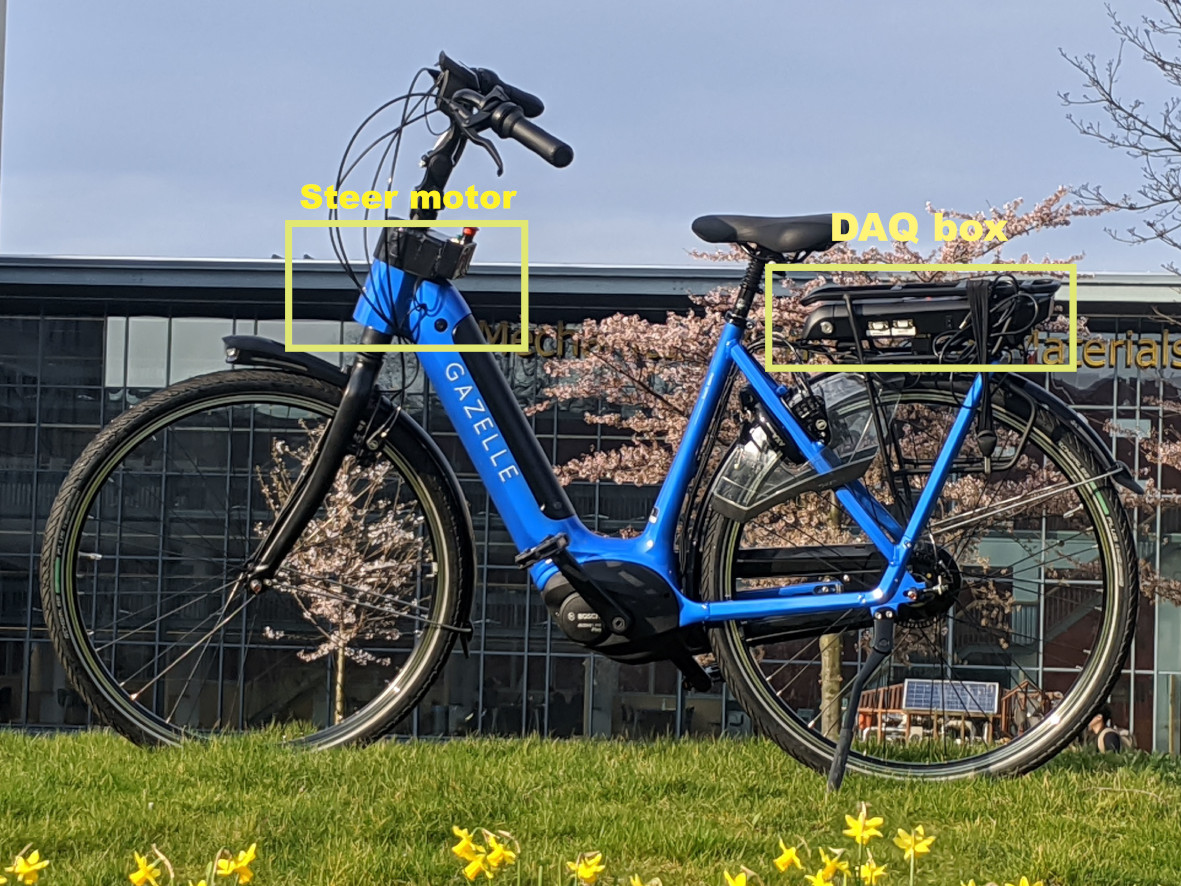
\includegraphics[width=70mm]{figures/balance-assist-bicycle.jpg}
  \caption{Balance assist bicycle prototype with electric motor in the steering
    column and data acquisition and control electronics mounted in the rear
    rack.}
  \label{fig:balance-assist-bicycle}
\end{figure}

In the early years of developments in automatic control, \citep{Whipple1899}
not only derived the correct equations of motion of the bicycle but realized
and showed that roll motion feedback can stabilize a bicycle. Much later,
attempts at automatic roll stabilization of single track vehicles began in
earnest after predictive motorcycle models were developed and refined in
throughout the 1970s. \Citet{vanZytveld1975} was influenced by Whipple's work
and seems to be the first to attempt to robotically stabilize a small motorbike
with a controlled inverted pendulum that mimicked rider lean, but he was not
successful in demonstrating what his theoretic control model correctly
predicted. In his model, he recognized that feedback of the vehicle roll angle
and angular rate was essential to stabilize the vehicle. It was not until the
early 1980s that \cite{Nagai1983} successfully demonstrated balancing a robotic
bicycle on a treadmill with both steering control and a laterally moving mass.
Ruijs and Pacjecka followed this by demonstrating an automatically balanced
motorcycle~\citep{Ruijs1986} and they did so with a steering motor. Ruijs and
Pacejka clearly showed that steer torque driven by roll angle feedback
stabilizes the capsize mode, roll angular rate feedback stabilizes the weave
mode, and steer angular rate feedback stabilizes the wobble mode. They also
proposed how the gains must change with respect to vehicle speed for favorable
control at all speeds. This roll motion feedback is the simplest controller
that can stabilize a single track vehicle above a minimum speed when one is not
concerned with wobble instabilities. Ruijs and Pacejka's work was not
particularly concerned with low speed stability and their vehicle was fully
automatic, no human rider was involved. Many more automatically balanced single
track vehicles have been demonstrated over the last 40 years, but none have
demonstrated that increasing low speed stability can assist in balancing and
possibly reduce single actor falls. Most of these robotic bicycle and
motorcycle designers did not intend for a human rider to also control the
stabilized vehicle. Nevertheless, an automatically stabilized bicycle can be
controlled by a human rider if the motor controlled steer torque and the rider
applied steer torque act on the steer in parallel.  The effect of this
automatic control gives the ability to change the dynamics, up to some limits,
of the human-controlled plant. In our prior study~\citep{Alizadehsaravi2023},
we demonstrate reduced motion during distractions due to the balance assist but
contrarily researchers with a similar vehicle recently showed rider
dissatisfaction with the stabilization~\cite{Hanakam2023}.

The linear Carvallo-Whipple bicycle model~\citep{Carvallo1899,Whipple1899} is
the simplest bicycle model that exhibits non-minimum phase behavior and
self-stability. The bicycle model is ideal for showing the effect of a roll
motion feedback driven steer motor on the dynamics. The linear version of this
model can be described by the fourth order state space
equations~\citep{Meijaard2007}:
%
\begin{align}
  \dot{\vec{x}} = \mathbf{A} \vec{x} +
  \mathbf{B}
  \vec{u}
  \textrm{ where }
  \vec{x} = \begin{bmatrix} \phi \\ \dot{\phi} \\ \delta \\ \dot{\delta} \end{bmatrix}
  \textrm{ and }
  \vec{u} = \begin{bmatrix} T_{\phi} \\ T_{\delta} \end{bmatrix}
  \textrm{.}
\end{align}
%
The states are the roll angle \(\phi\) and steer angle \(\delta\) along with
their derivatives and the inputs are roll torque \(T_\phi\) and steer torque
\(T_\delta\). The state \(\mathbf{A}\) and input \(\mathbf{B}\) matrices are
functions of the equilibrium forward speed \(v\) and  are otherwise populated
with expressions that are functions of the geometric and inertial parameters of
the nonholonomic multibody system made up of four rigid bodies: two wheels,
front frame, and rear frame.

If the steer torque is the sum of the (h)uman applied torque and the (m)otor
applied torque \(T_\delta = T_\delta^\textrm{h} + T_\delta^\textrm{m}\),
\(\mathbf{B} = \begin{bmatrix} \vec{B}_\phi \quad \vec{B}_\delta
\end{bmatrix}\), and \(T_\delta^\textrm{m} = -k_{\dot{\phi}} \dot{\phi}\) then
the human controlled plant takes the form:

\begin{align}
  \dot{\vec{x}} = \left(\mathbf{A} -
  \vec{B}_\delta
  \left[0 \quad k_{\dot{\phi}} \quad 0 \quad 0\right]
\right)
  \vec{x} + \mathbf{B} \begin{bmatrix} T_{\phi} \\ T_\delta^\textrm{h} \end{bmatrix}
\end{align}

The state matrix \(\mathbf{A}\) and input matrix \(\mathbf{B}\) are both
functions of the equilibrium speed \(v\) and \(k_{\dot{\phi}}\) can be selected
such that the eigenvalues of \(\left(\mathbf{A} - \vec{B}_\delta\left[0 \quad
k_{\dot{\phi}} \quad 0 \quad 0\right] \right)\) have negative real parts for
\(v_{min} < v < v_\textrm{capsize}\) where \(v_{min}\) is the lowest stable
speed given \(k_{\dot{\phi}}\) and \(v_\textrm{capsize}\) is the speed at which
the uncontrolled bicycle's capsize mode goes unstable. With gain scheduling
with respect to \(v\), the speed range where the bicycle is stable can be
maximized within any physical actuator magnitude and bandwidth limits.
\citet{Schwab2008} elaborates on some of the possibilities in scheduling the
gains for such a controller and shows that a linear scheduling with respect to
speed can give satisfactory stability.

In this paper, we test whether a linearly gain scheduled steer motor controlled
bicycle, that is stable in a large low speed range when riderless, is
beneficial in helping to prevent the rider from falling. We test this by
applying varying magnitude mechanical perturbations to the handlebars while the
rider is cycling on a treadmill. We assess the difference in the rider's
probability of falling with the balance assist steer motor system on and off.

\section{Methods}
%
\subsection{Bicycle}
%
We modified a standard electric bicycle (Gazelle Grenoble C7\todo{Double check
this is the right model}, Dieren, The Netherlands) with a custom motor in the
steering assembly capable of applying up to 7~\si{\newton\meter} of torque
between the head tube and steer tube, see
Figure~\ref{fig:balance-assist-bicycle}.  A custom motor controller converts
the commanded torque to applied torque. We measure the speed of the rear wheel
with an encoder (Magura XXX) and measure the body fixed roll rate of the
bicycle with a MEMs rate gyroscope (CRS 03-02s, Silicon Sensing, United
Kingdom).  \todo{Do you mean the gyro inside the bicycle or the external?
Currently filled in the data of the external one. Not sure what make and model
is inside the bicycle} The balance assist control algorithm is implemented on a
microprocessor (Teensy, PJRC, USA) and data from all sensors is logged with a
CAN bus (CanEdge2, CSS Electronics, Denmark) at approximately 100 Hz.
\todo{Sample rate is not the same for each sensor: wheel speed, imu = 1ms,
steer torque command is updated every 10ms, can log is written every 10ms}

\subsection{Balance Assist Control}
%
We use a forward speed \(v\) gain scheduled proportional roll rate feedback
controller to stabilize the bicycle. The commanded steer torque
\(T^\textrm{m}_\delta\) from the steer motor follows the control law
%
\begin{align}
  T^\textrm{m}_\delta = -k_{\dot{\phi}}\dot{\phi} = g(v_{weave} - v)\dot{\phi}
\end{align}
%
where 4.7~\si{\meter\per\second} is the weave critical speed predicted from the
open loop bicycle rigid-rider dynamics. We use \(g=8\) and \(g=10\) as gain
values during the experiments. Scaling the proportional feedback gain linearly
with respect to speed stabilizes the normally unstable weave mode of the
bicycle from speeds of X~\si{\kilo\meter\per\hour} to
X~\si{\kilo\meter\per\hour} as shown in Figure~\ref{fig:eigenvalues}.

\begin{figure}
  \centering
  \subcaptionbox{}{
    \includegraphics[width=100mm]{figures/uncontrolled-eig-vs-speeds.png}
  }
  \subcaptionbox{}{
    \includegraphics[width=100mm]{figures/balance-assist-controllers-eig-vs-speeds.png}
  }
  \caption{Uncontrolled (a) and controlled (b) root locus of eigenvalue
    components (real: solid, imaginary: dashed) plotted versus speed. Vertical
    blue lines indicate the two speeds we perform experiments at. Green shaded
    region is the linear stable range.}
  \label{fig:eigenvalues}
\end{figure}

\todo[inline]{Decide on what physical parameters to use.}

\subsection{Perturbations}
%
We apply external longitudinal forces to the ends of each handlebar using an
adapted Bump'Em system~\cite{Tan2020} which is designed with four motors
working in tandem, Figure~\ref{fig:setup-diagram}. The four motors are
programmed to apply a light force at all times to keep the ropes taught and to
track a commanded force profile using a PID controller running on a
microprocessor (Arduino Mega 2560, Italy). We measure the force applied by each
motor at the handlebar via four inline load cells, each with a max load of
250~\si{\newton}. The left rear load cell  was damaged during pilot
experiments, and is replaced by a load cell with a max load of
500~\si{\newton}. The commanded force profiles are designed to apply an
external pulsive torque to the front assembly (handlebars, forks, wheel) at
magnitudes varying from 20 to 200~\si{\newton} per motor.  This results in a
torque between 16 and 160~\si{\newton\meter}. The four motors are arranged at
the four corners of a 1~\si{\meter} wide treadmill (EC-90 Flat, Maxon Group,
Switzerland) that can reach speeds of 18~\si{\kilo\meter\per\hour}.  The
general design is described in detail in the Van De Velde's MSc
hesis~\citep{vandeVelde2022a} and the physical arrangement  is shown in
Figure~\ref{fig:participant-in-set-up}. Our modifications relative to that
described in the thesis include simplifying the controller with a inexpensive
microcontroller and the use of a simpler safety harness.
Figure~\ref{fig:perturbation_0} shows an example perturbation.
%
% NOTE : I get a compile error with the \protect calls here, not sure why.
\begin{figure}
  \centering
  \subcaptionbox{A participant on the bicycle in the safety harness with the
    Bump'Em motor lines attached to the ends of the
    handlebars.\protect\label{fig:participant-in-set-up}}
    {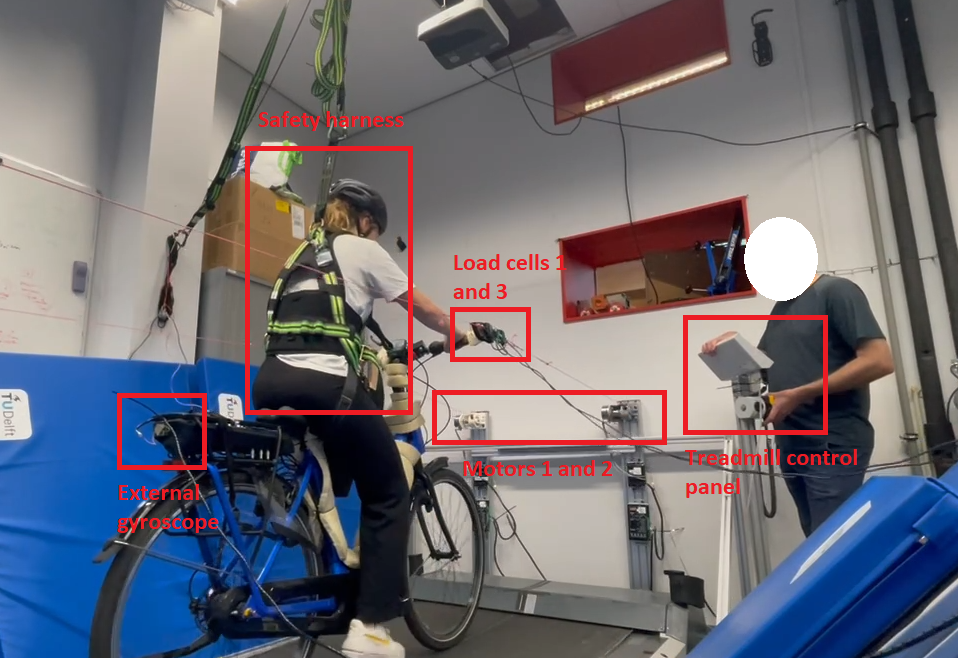
\includegraphics[width=75mm]{figures/participant-in-set-up.png}}
  \subcaptionbox{Top view diagram of bicycle handlebar perturbation
    system.\protect\label{fig:setup-diagram}}
    {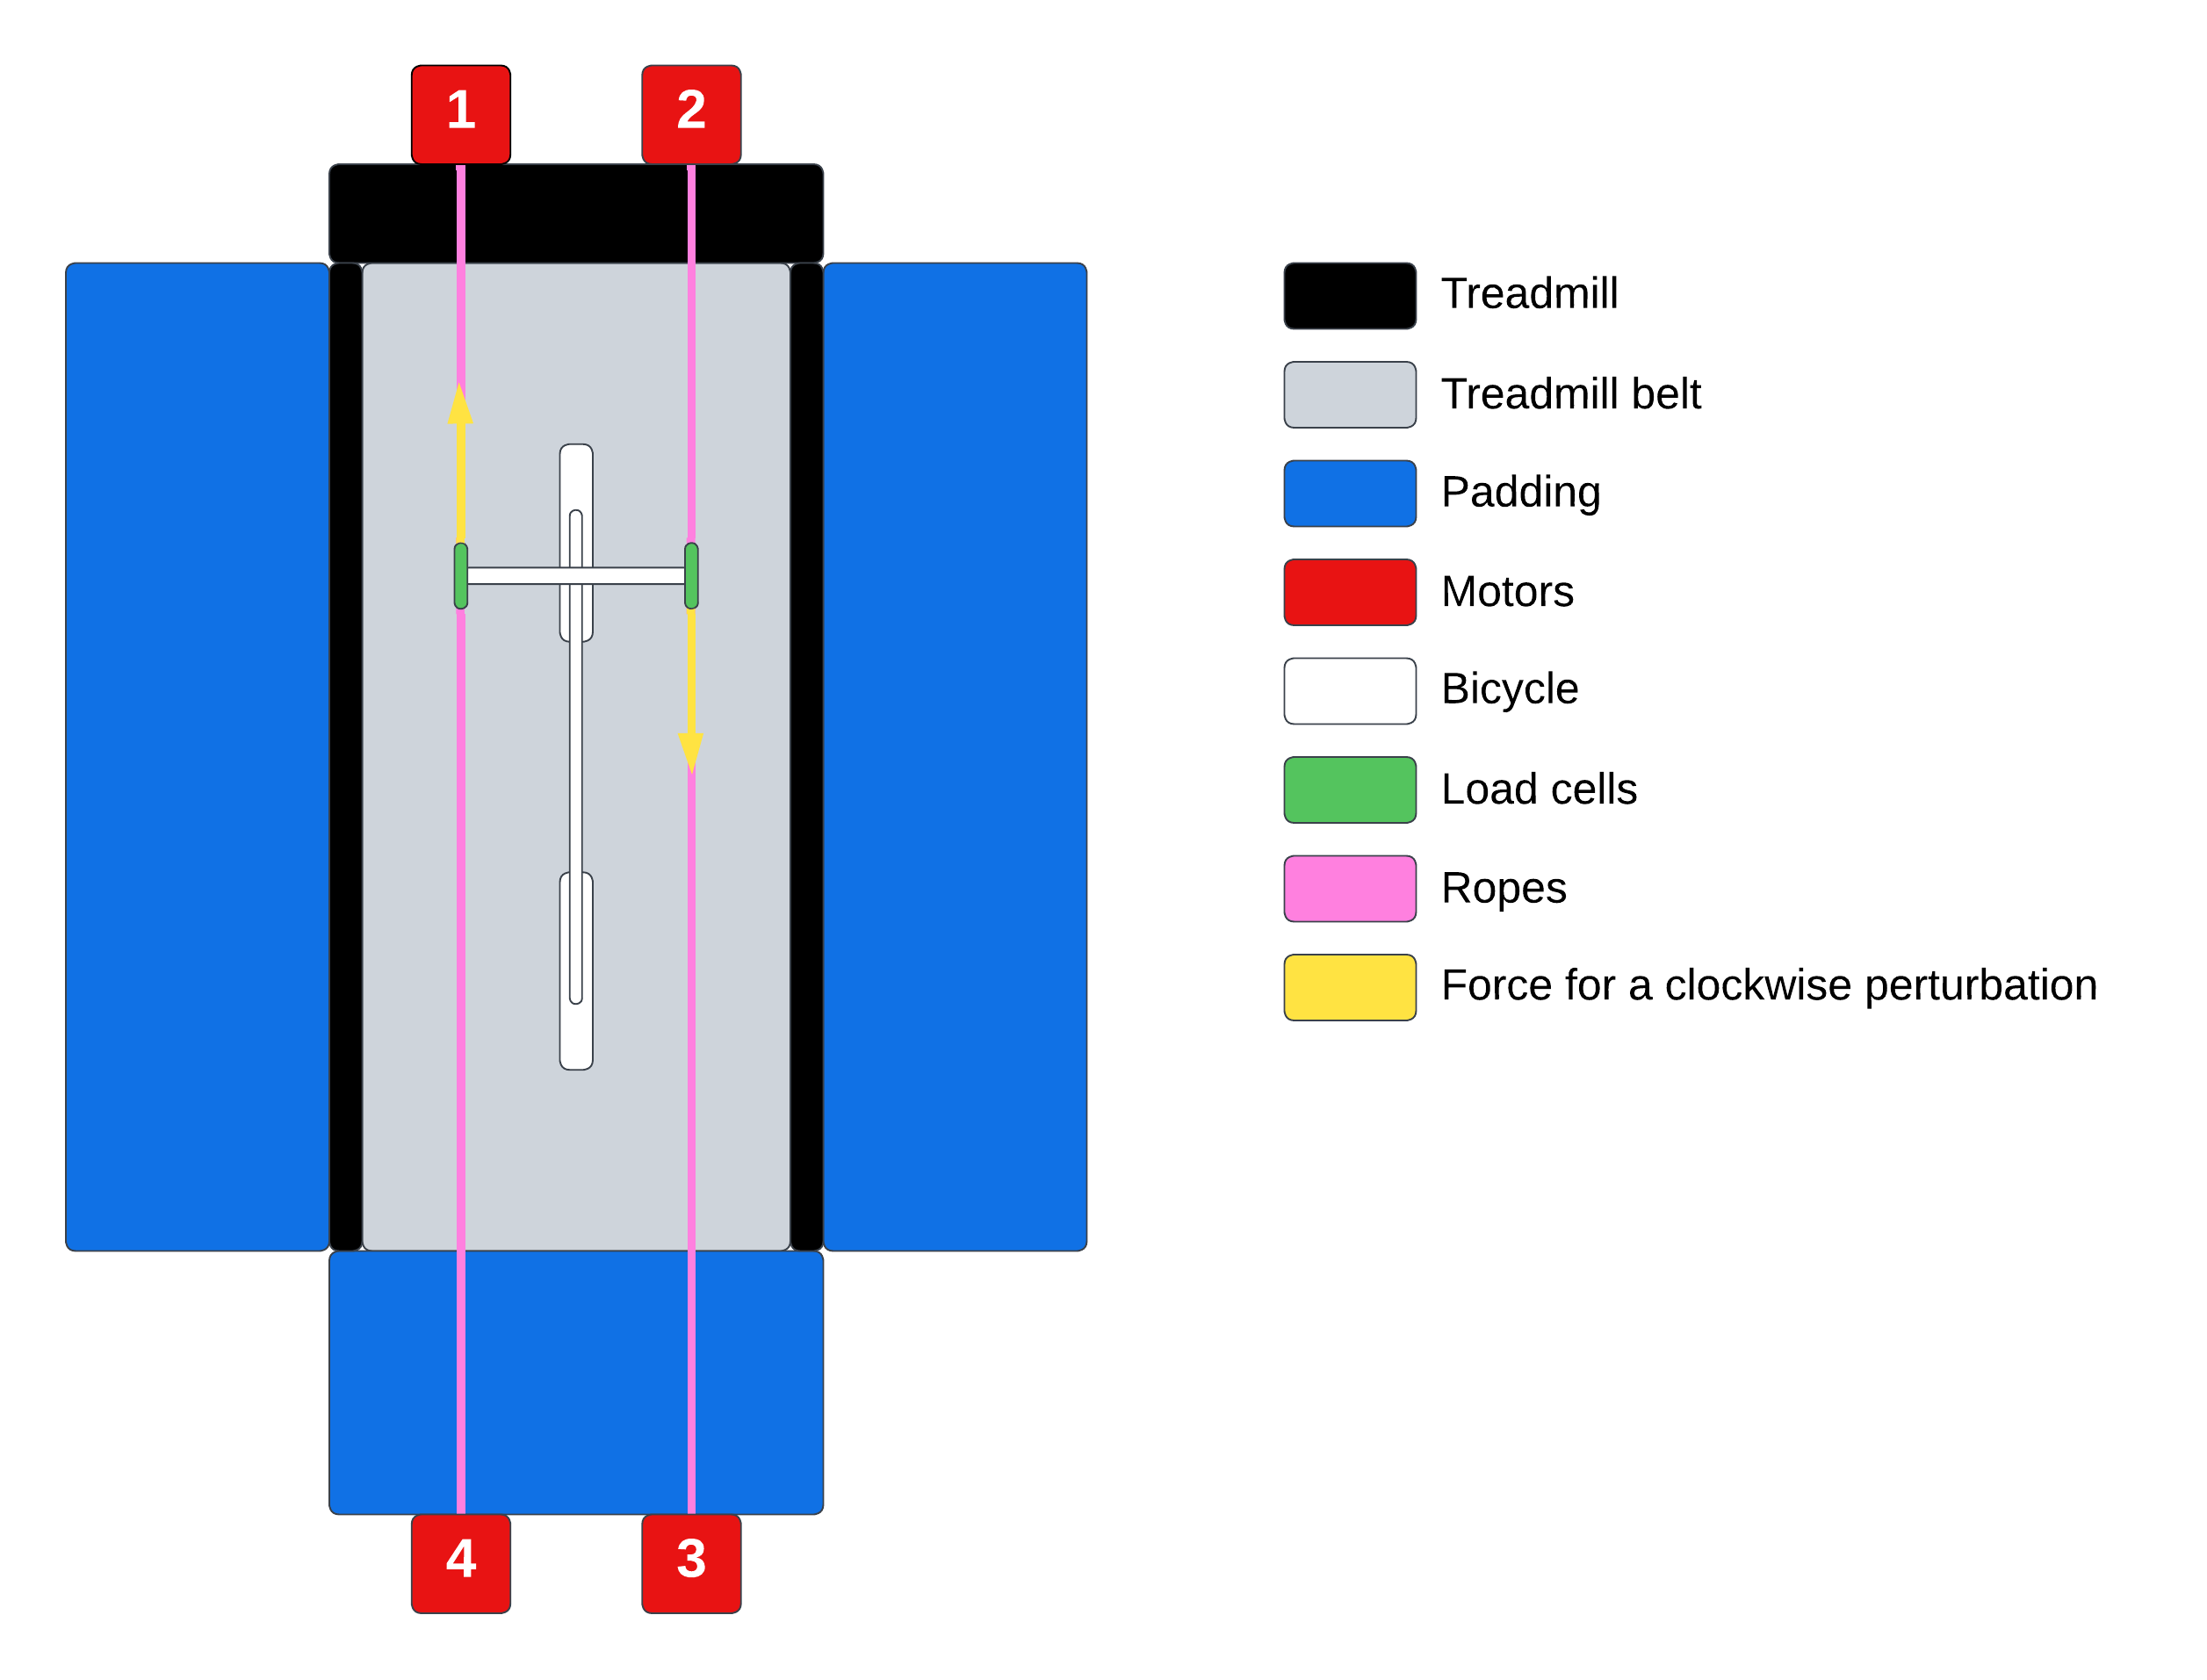
\includegraphics[width=65mm]{figures/setup-diagram.png}}
  \caption{Diagrams showing the Bump'Em system arranged to apply handlebar
    perturbations.}
  \label{fig:experimental-setup}
\end{figure}

\subsection{Protocol}
%
We recruited 26 able-bodied young adults (20-36 years old) to participate in
the experiments. The subjects all were confident in their cycling skills and
had cycled at least once in the last month. Eleven subjects performed the
experiments at 1.7~\si{\meter\per\second} (6~\si{\kilo\meter\per\hour}) and
fifteen subjects performed the experiments at 2.8~\si{\meter\per\second}
(10~\si{\kilo\meter\per\hour}). All subjects consented to the experiment and
could decline to continue at any time. The study was approved by Delft
University of Technology's Human Research Ethics Council (\#3897).

\todo[inline]{Include the average age, mass, height and standard deviation if
we recorded those.}

The subjects were divided into two groups. The first group performed the
protocol at a belt speed of 2.8~\si{\meter\per\second}
(10~\si{\kilo\meter\per\hour}) with the controller gain at $g=8$ and the second
group performed the protocol at a belt speed of 1.7~\si{\meter\per\second}
(6~\si{\kilo\meter\per\hour}). The 10~\si{\kph} group's experiments occurred 2
weeks before the 6~\si{\kilo\meter\per\hour} group.

Subjects wore a helmet and fall safety harness attached to the ceiling
Figure~\ref{fig:participant-in-set-up}. We allowed them to practice riding on
the treadmill until they indicated they were comfortable enough to have
perturbations applied. For most, this was less than a 10~\si{\minute} warm up.
We then asked the rider to ride for 90~\si{\second}, attempting to maintain the
location of their front wheel on the center line of the treadmill. \todo{The
  results from this are not included because the balance-assist was turned on
for some participants} We define a ``fall'' on the treadmill by two criteria:
the rider removes their foot from the pedal and places it on the ground or the
bicycle wheel exceeds the width of the treadmill. We then applied perturbations
in random directions (clockwise or counter clockwise), starting at
20~\si{\newton} and increasing the magnitude by 30~\si{\newton\meter} until the
participants falls.  Figure~\ref{fig:perturbation-sequence} shows an example
result of a perturbation.  We log the magnitude that causes the first fall to
characterize that subject's nominal fall threshold. Following this we apply 20
perturbations of varying magnitudes to the cyclist while they ride at a
constant speed and record which perturbations cause a fall. We let the cyclist
rest and then perform another 20 perturbations. We randomize whether the
balance assist system is on or off during the first or second set of
perturbations.

%
\begin{figure}
  \centering
  \subcaptionbox{Start}{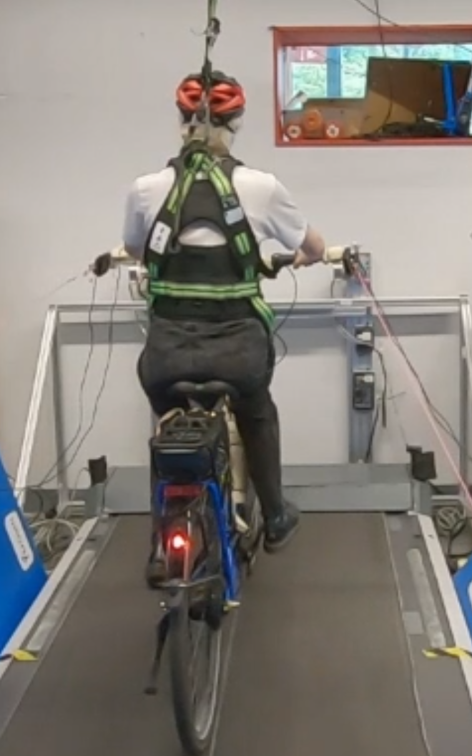
\includegraphics[width=40mm]{figures/start.png}}
  \subcaptionbox{During}{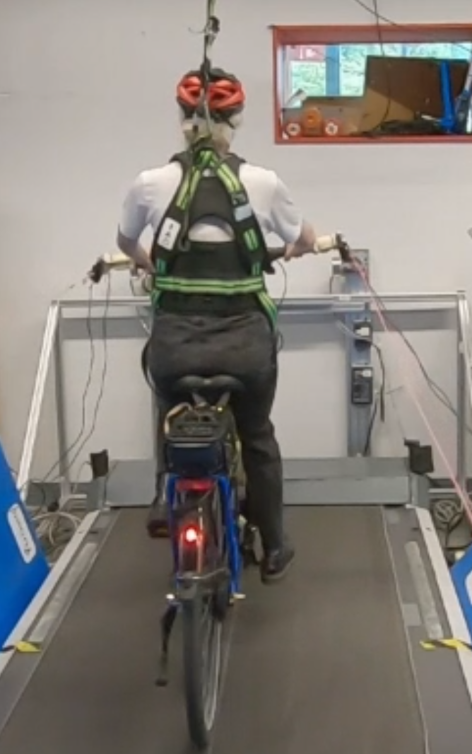
\includegraphics[width=40mm]{figures/during.png}}
  \subcaptionbox{After}{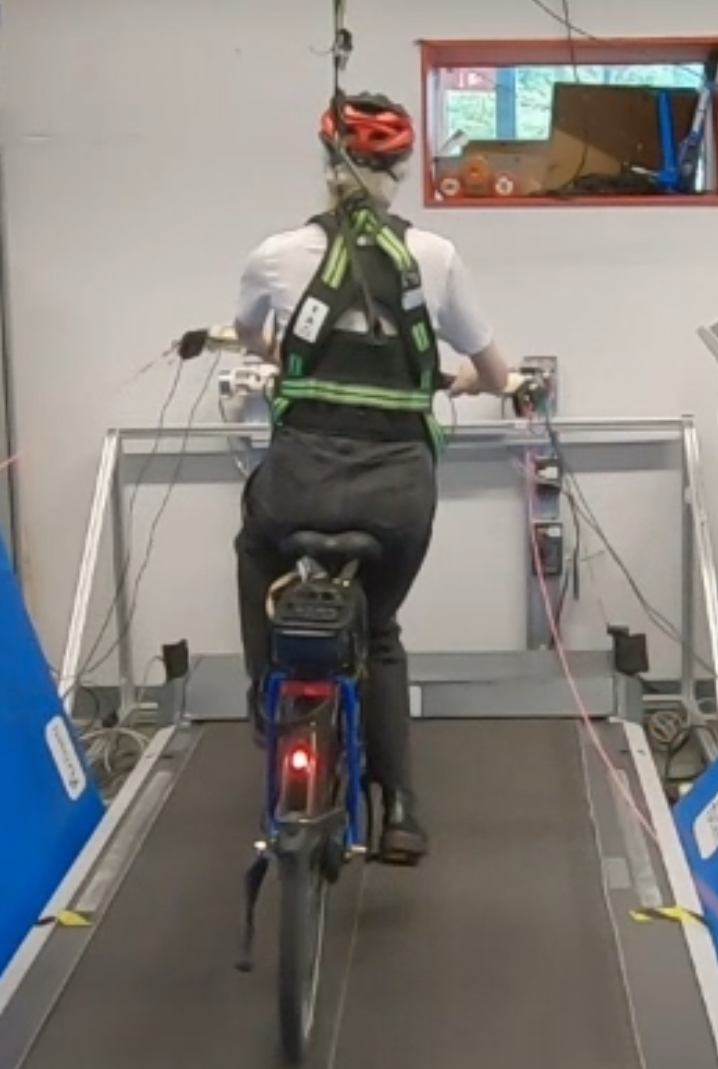
\includegraphics[width=40mm]{figures/after.png}}
  \subcaptionbox{Recovery}{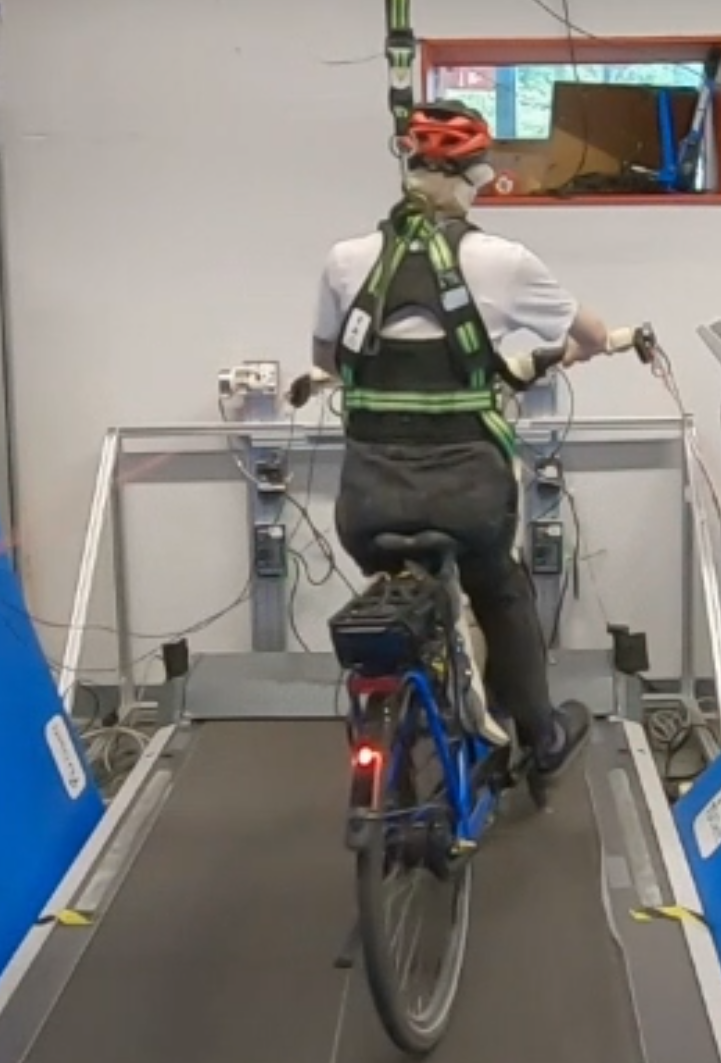
\includegraphics[width=40mm]{figures/recovery.png}}
  \caption{Video frames depicting the application of a perturbation and the
  rider's response and recovery.}
  \label{fig:perturbation-sequence}
\end{figure}

Following the initial threshold determination, we choose perturbation forces
according to a random and adaptive staircase procedure applying perturbations
above and below the initial perturbation threshold, while allowing small
progression of the perturbation threshold to accommodate learning effects. The
goal of this adaptive staircase procedure is to have participants fall for
approximately 50\% of the time. The procedure consists of twenty perturbations
per condition. Participants undergo two conditions: twenty perturbations with
the balance-assist turned on and twenty perturbations with the balance-assist
turned off.

Five possible perturbation forces are determined based on the initial
perturbation threshold estimate: the initial estimate itself, two perturbations
lower than the initial estimate and two perturbations higher than the initial
estimate.  The five possible perturbations are separated by 10 N steps. For
example, if the initial estimate of the perturbation threshold of a participant
is 80~\si{\newton}, the five possible perturbations are 60, 70, 80, 90 and
100~\si{\newton}. Which one of these five perturbations is chosen is
determined at random. If the perturbation results in a fall, the estimate of
the perturbation threshold is decreased with 10~\si{\newton}, and vice versa
if the perturbation did not result in a fall. Five new possible perturbation
forces are determined around the updated perturbation threshold, and a new
perturbation is selected at random. This process iterates until twenty
perturbations are applied.

\subsection{Measurements}
%
We measure the time histories of the Bump'Em delivered perturbation forces and
the bicycle's steer angle, roll angle, roll angular rate, and forward speed.
Figure~\ref{fig:perturbation_0} shows an example perturbation force
measurement compared to our Bump'Em controller command.
%
\begin{figure}
  \centering
  \includegraphics[width=140mm]{figures/torque_angle_perturbation_10.png}
  \caption{Motor force and resulting  steer torque perturbation based on an 80N
    counterclockwise applied force.}
  \label{fig:perturbation_0}
\end{figure}

Based on findings from measuring riders without balance
assist~\cite{Haitjema2023a}, we calculate several variables that we hypothesize
may influence fall probability. We use the angular impulse \(L\) of the
perturbation forces over a 0.3~\si{\second} duration to characterize the
magnitude of delivered perturbation. The duration is selected based on the
duration of the commanded force and is calculated as follows:

\begin{align}
  L =
  \int_{0\si{\second}}^{0.3\si{\second}} \frac{l}{2}(F_r + F_l) dt
  =
  \int_{0\si{\second}}^{0.3\si{\second}} \frac{l}{2}\left[(F_{rf} - F_{rr}) + (F_{lf}
  - F_{lr})\right] dt
  \textrm{.}
\end{align}

At the initiation of each perturbation we log the steer and roll angles to
characterize the configuration of the bicycle when perturbed. The gain setting
on the balance assist controller indicates if the assistance is off \(g=0\) or
on at two different levels: low \(g=8\) or high \(g=10\). A recovery from the
perturbation is successful if the person neither put their foot down onto the
treadmill surface or either wheel of the bicycle exits the width of the
treadmill belt. We record this as a binary variable \(f\). All measured
variables are reported in Table~\ref{tab:raw}.
%
\begin{table}
  \centering
  \caption{Raw measurements taken during each trial. ``Fall outcome'' and
    ``Perturbation order number'' are recorded per perturbation instance.}
  \begin{tabular}{llll}
    \toprule
    Measure & Variable & Units & Sensor \\
    \midrule
    Balance Assist Gain & \(k\) & TODO & NA \\
    Bicycle Speed & \(v\) & \si{\meter\per\second} & wheel encoder \\
    Fall outcome & \(f\) & boolean & NA \\
    Force \(l\)eft/\(r\)ight,\(f\)ront/\(r\)ear & \(F_{lf},F_{rf},F_{lr},F_{rr}\) & \si{\newton} & load cell\\
    Perturbation Order Number & \(j\) & integer & NA\\
    Roll Angle & \(\phi\) &  \si{\degree} & Kalman estimate~\citep{Gabriel2023} \\
    Roll Angular Rate & \(\dot{\phi}\) &  \si{\degree\per\second} & rate gyroscope \\
    Steer Angle & \(\delta\) & \si{\degree} & steer tube encoder \\
    \bottomrule
  \end{tabular}
  \label{tab:raw}
\end{table}

\subsection{Statistics}
%
We test the hypothesis that the balance assistance controller will reduce the
probability of falling when perturbed externally at the handlebar. We have a
single binary fall outcome variable \(f\) that is dependent on several possible
explanatory independent variables, one of which is the binary balance
assistance (on or off). See Table~\ref{tab:stat-model-variables} for all of the
variables.
%
\begin{table}
  \centering
  \caption{Statistical model variables.}
  \label{tab:stat-model-variables}
  \begin{tabular}{lll}
    \toprule
    Variable & Units & Description \\
    \midrule
    \(L\) & \si{\newton\meter\second} & angular impulse of perturbation torque \\
    \(c\) & integer & order number of perturbation \\
    \(k\) & TODO & gain of balance assist control \\
    \(\delta_0\) & \si{\degree} & steer angle at start of perturbation \\
    \(\phi_0\) & \si{\degree} & roll angle at start of perturbation \\
    \(v\) & \si{\meter\per\second} & forward speed (1.7 or 2.8) \\
    \(f\) & boolean & outcome of perturbation: did not fall, did fall \\
    \bottomrule
  \end{tabular}
\end{table}

We evaluate this hypothesis using a multivariate logistic regression model that
takes the general form
%
\begin{align}
  f_{ij} | p_{ij} \sim \textrm{Bern}(p_{ij}) \textrm{.}
\end{align}
%
Fall outcome \(f_{ij}\) is the binary outcome of perturbation \(j\) on
participant \(i\) which follows a Bernoulli distribution given the probability
\(p_{ij}\) that a fall occurs. The log-odds of the probability is then a linear
function of our independent variables with \(\beta\) as the intercept and
\(\alpha_k\) as the linear coefficients to the independent variables
\(x_{ij}^k\), i.e. all variables in Table~\ref{tab:stat-model-variables} except
\(f\).
%
\begin{align}
  \log \left(\frac{p_{ij}}{1-p_{ij}} \right) =
  \beta + \sum_{k=0}^{K} \alpha_k x_{ij}^{k}
  \label{eq:log-regress}
\end{align}

Before fitting the model, we scale each \(x_{ij}^k\) such they they have a mean
of zero and a standard deviation of one by cluster-mean centering, as
recommended by \cite{Enders2007}, with clusters being an individual subject.
The clusters are all data from an individual subject because we are only
interested in the association between the state of the balance-assist system
and the outcome of the perturbation. We expected there to be a variation
between participants in how well they are able to resist the perturbation.
However, this was not true. Cluster-mean centering shows there to be no
variation between participants. This allowed us to stick with a simple
single-level logistic regression model, instead of a multilevel model. This
left us with angular impulse, perturbation order, balance assist state, and
roll \& steer angles at the time of perturbation as independent variables. We
also include interaction effects between the balance assist state and the other
four variables.

We divide the analysis into two separate model evaluations, one for the
6~\si{\kph} \(g=10\) trials and one for the
10~\si{\kph} \(g=8\) trials and we evaluate our hypothesis for
each set of data.

\section{Results}
%
The coefficient estimates for a single-level logistic regression at
6~\unit{\kph} with gain $g=10$ are shown in
Table~\ref{tab:freq-coefs-6}. The angular impulse, perturbation order, and
balance assist state are all statistically significant predictors. Larger
angular impulse increases the probability to fall and enduring more
perturbations or having the balance assist on, decrease the probability to
fall.  The associated multiplicative change in odds are shown in
Table~\ref{tab:freq-coefs-6}.
%
\begin{table}
  \centering
  \caption{Logistic regression coefficient estimates at
    6~\unit{\kilo\meter\per\hour} and gain $g=10$. Multiplicative change in
    odds of predictor variables at 6 \unit{\kilo\meter\per\hour} and gain
    $g=10$ based on frequentist single-level logistic regression.}
  \label{tab:freq-coefs-6}
  \begin{tabular}{lrrrrrr}
    \toprule
    Variable & \(\alpha_k\) & SE & \(p\)-value & $e^{\alpha_k}$ & 2.5\% & 97.5\% \\
    \midrule
    Intercept & -0.29 & 0.17 & 0.09 & 0.75 & 0.53 & 1.05 \\
    Angular impulse & 1.69 & 0.27 & 0.00 & 5.40 & 3.18 & 9.16 \\
    Perturbation order & -0.77 & 0.22 & 0.00 & 0.46 & 0.30 & 0.72 \\
    Balance assist state & -0.64 & 0.27 & 0.02 & 0.53 & 0.31 & 0.89 \\
    Roll angle & -0.25 & 0.21 & 0.24 & 0.78 & 0.51 & 1.18 \\
    Steer angle & -0.14 & 0.21 & 0.51 & 0.87 & 0.58 & 1.32 \\
    Balance-assist on $\times$ roll angle & 0.52 & 0.34 & 0.12 & 1.68 & 0.86 & 3.29 \\
    Balance-assist on $\times$ steer angle & -0.41 & 0.34 & 0.22 & 0.66 & 0.34 & 1.28 \\
    Balance-assist on $\times$ angular impulse & 0.41 & 0.41 & 0.32 & 1.51 & 0.67 & 3.38 \\
    Balance-assist on $\times$ perturbation order & -0.53 & 0.34 & 0.12 & 0.59 & 0.30 & 1.15 \\
    \bottomrule
  \end{tabular}
\end{table}

The coefficient estimates for a single-level logistic regression at
10~\si{\kilo\meter\per\hour} with gain $g=8$ are shown in Table
\ref{tab:freq-coefs-10}. The angular impulse and perturbation order are
statistically significant predictors. Larger angular impulse increases the
probability to fall and enduring more perturbations decreases the probability
to fall.

\begin{table}
  \centering
  \caption{Logistic regression coefficient estimates at
    10~\unit{\kilo\meter\per\hour} and gain $g=8$.  Multiplicative change in
    odds of predictor variables at 10 \unit{\kilo\meter\per\hour} based on
    frequentist single-level logistic regression. and 5\% confidence intervals
  of MCiO.}
  \label{tab:freq-coefs-10}
  \begin{tabular}{lrrrrrr}
    \toprule
    Variable & \(\alpha_k\) & SE & \(p\)-value & $e^{\alpha_k}$ & 2.5\% & 97.5\% \\
    \midrule
    Intercept                                     & -0.24 & 0.16 & 0.13 & 0.78 & 0.57 & 1.07 \\
    Angular impulse                               & 2.39  & 0.29 & 0.00 & 10.92 & 6.23 & 19.13 \\
    Perturbation order                            & -1.16 & 0.21 & 0.00 & 0.31 & 0.21 & 0.48 \\
    Balance-assist on                             & -0.44 & 0.24 & 0.07 & 0.64 & 0.40 & 1.03 \\
    Roll angle                                    & 0.27  & 0.22 & 0.22 & 1.31 & 0.85 & 2.04 \\
    Steer angle                                   & -0.37 & 0.24 & 0.12 & 0.69 & 0.43 & 1.10 \\
    Balance-assist on $\times$ roll angle         & -0.61 & 0.34 & 0.08 & 0.54 & 0.28 & 1.07 \\
    Balance-assist on $\times$ steer angle        & 0.56  & 0.35 & 0.11 & 1.76 & 0.88 & 3.50 \\
    Balance-assist on $\times$ angular impulse    & 0.46  & 0.44 & 0.29 & 1.59 & 0.68 & 3.74 \\
    Balance-assist on $\times$ perturbation order & -0.37 & 0.32 & 0.25 & 0.69 & 0.37 & 1.30 \\
    \bottomrule
  \end{tabular}
\end{table}

Turning the balance-assist system on significantly \((p<0.05)\) reduces the
odds that a pertubation results in a fall occurs while cycling at a speed of
6~\si{\kph}.  Figure~\ref{fig:probability-6kph} visualizes the probability of
falling as a function of the mean and centered angular impulse per participant
while keeping all other explantory factors at their centered mean values. This
figure is derived by setting all explanatory variables to there mean and
calculating the probality from Eq~\ref{eq:log-regress} for only change in
angular impulse given the estimates in Table~\ref{tab:freq-coeffs-6} which
indicate that the balance-assist system halves (0.53) the odds that a
perturbation results in a fall. This figure shows that for relatively large
impulses the probability to fall is unity for both states of balance assist on
and off. And for relatively small impulses the probability to fall is zero for
both states. But for impulses in the magnitude region (-1 to 0.5 STD) around
the mean-centered fall threshold, the probability of falling is significantly
lowered. The skewedness of the probaility curves arrives from the interaction
effects\todo[inline]{check this and think about it}.

\todo{Discuss the 10 kph finding}

but at 10~\si{\kph} that is not the case \((p=0.07)\).

\begin{figure}
  \centering
  \subcaptionbox{6~\si{\kph}\label{fig:probability-6kph}}{
    \includegraphics[width=120mm]{figures/predicted_fall_probability_6kmh.png}
  }
  \subcaptionbox{2.8~\si{\mps}}{
    \includegraphics[width=120mm]{figures/predicted_fall_probability_10kmh.png}
  }
  \caption{Comparison of predicted fall probability for balance-assist on or
    off All other predictor variables are fixed at zero, except for the
    interaction effect between the balance-assist and the angular impulse. The
    x axis is standard deviation around the mean (all perturbations), centered
    per participant.}
  \label{fig:probability}
\end{figure}

\section{Discussion}
%
The probability that a fall occurs depends on the values of all the independent
variables in Table~\ref{tab:stat-model-variables}, but we can visualize the
effect of one or two variables (e.g. Figure~\ref{fig:probability}) to gain
some insight.
But to interpret the results in Tables~\ref{tab:freq-coeffs-6} and
\ref{tab:freq-coeffs-10} it is important to understand the relationship between
probability and odds.
The estimate in Table~\ref{tab-freq-coeffs-6} shows that the balance assist
system halves the odds that a perturbation results in a fall
(MCiO=0.53)~\todo{Make a variable for MCiO}.
This means if the odds are a 1000:1, turning on the balance-assist system
reduces the odds to 500:1.
However, the probability that a fall occurs is only reduced from $0.999$ to
$0.998$ in that case.
If the odds that a fall will occur are smaller, halving the odds has a larger
influence on the fall probability.
For example, if the odds that a fall occurs is two, halving it to one reduces
the probability from $0.66$ to $0.50$.
This can be seen in Figure~\ref{fig:probablity} which shows the fall
probability as a function of the magnitude of the normalized angular impulse
for both speeds.
The difference in probability between the balance-assist on/off case becomes
insignificant outside of approximately \(\pm1\) standard deviation of the
average angular impulse.
This means that the balance assist is most effective for perturbations close to
the subject's personal threshold between falling or recovery and that large
perturbations will make you fall regardless of the balance assist's help.

\todo{Consider making a specific value of calcualting the probabilty for a set
of inputs to the regression model.}

To illustrate the effect of the balance-assist system on fall probability, we will
give an example of how the data collected during the experiments is used to predict
fall probability. We use \ref{eq:log-regress} and the coefficients in 
\ref{tab:freq-coefs-6}. For simplicities sake, the interaction effects are not included.
Let's assume that the mean angular impulse $\bar{L}$ of all the perturbations applied to 
a participant is 100~\si{\newton}, and the standard deviation $\sigma^{L}=15$. The centred
and scaled angular impulse can be calculated by substracting $\bar{L}$ from the applied
angular impulse $L$, and dividing this by $\sigma^{L}$. The same applies for the 
perturbation order $c$, initial roll angle $\phi_0$ and initial steer angle $\delta_0$.
If we take the coefficients estimated for cycling at 6~\si{\kilo\meter\per\hour}, the
log-odds of falling can be calculated as follows.

\begin{align}
	\log \left( \frac{p_{ij}}{1-p_{ij}} \right) & = \beta + \sum_{k}^{k=0}\alpha_k 
	\frac{x_{ij}^{k}-\bar{x_{ij}^{k}}} {\sigma^{x^{k}}} 
	& = -0.29 + 1.69\cdot\frac{110~\si{\newton} - 115\si{\newton}}{15\si{\newton}} 
	-0.77\cdot\frac{10-20}{11.54} 
	-0.25\cdot\frac{-6\si{\degree}-2\si{\degree}}{10\si{\degree}} 
	-0.14\cdot\frac{1\si{\degree}+3\si{\degree}}{5\si{\degree}}
	-0.64\cdot s
	& = 1.42 -0.64 \cdot s
\end{align}

The state of the balance-assist $s$ is a binary variable. If the balance-assist is turned on, 
the log-odds that a fall occurs are decreased by 0.64. The odds and probability can be calculated:

\begin{align}
	\frac{p_{ij}}{1-p_{ij}} = e^{1.42-0.64s} = e^{1.42}\cdot e^{-0.64s} = 4.14 \cdot 0.53s
\end{align}

\begin{align}
	p_{ij}^{s=0} = \frac{4.14}{1 + 4.14} = 0.81
\end{align}

\begin{align}
	p_{ij}^{s=1} = \frac{4.14\cdot0.53}{1 + 4.14\cdot{0.53}]} = 0.69
\end{align}

Turning on the balance-assist system reduces the probability that the perturbation results in a 
fall from 0.81 to 0.69.

Angular impulse magnitude has the largest significant effect for predicting
fall probability, Tables~\ref{tab:freq-coeffs-6} and \ref{tab:freq-coeffs-10}.
An increase in angular impulse increases the fall probability both at 6 and
10~\si{\kph}. At 10~\si{\kph}, the multiplicative change in odds is
approximately twice as big as at 6~\si{\kph}. Thus, angular impulse is a more
important predictor at higher speeds compared to lower speeds. The reason for
this likely has to do with the width of the treadmill and may also be why
balance assist system did not have a statistically significant effect at
10~\si{\kph}. As a bicycle travels at higher speeds, the same perturbation
causes larger lateral deviations. At 10~\si{\kph} almost all falls were due to
the bicycle exiting the maximum width of the treadmill. If the same experiment
was performed on an infinite plane, the riders may have recovered from more
perturbations. At 6~\si{\kph} the riders could often recover in the allotted
treadmill width. Our results are very much dependent on the two modes of
falling with use: exit the treadmill width or foot is placed on the belt. Cycle
paths are a similar width as the treadmill, so rider's are often limited in
width when recovering from a fall.

\todo[inline]{Could show an impulse response in lateral deviation for different
speeds.}

An increase in the number of perturbation that a participant already
experienced, decreases the probability that a fall occurs. This is likely due
to the participants learning how to better recover from the perturbation over
the duration of the experiment. This effect is significant at both 6 and
10~\si{\kph}, and in the same order of magnitude. This suggests that the
learning effect that occurs during the experiment is not strongly dependent on
the speed.

Roll and steer angle are not a significant predictor of fall probability,
neither at 6 or at 10~\si{\kph}. We expected this to have an effect. If you are
in a rolled and steered state that is far from the upright equilibrium, then a
perturbation that further pushes you from the equilibrium should have some
additive or multiplicative effect on the resulting motion trajectory.

None of the interaction effects are statistically significant. That means that
whether the balance-assist system is on or off does not significantly change
the effect that the roll angle, steer angle, angular impulse, and perturbation
order have on the probability that a fall will occur.

Difficult to layer this onto the fall statistics, because we don't have the
details of how people fall. If such data existed we could make estimates on the
number of falls reduced if everyone road such a bike.

\section{Conclusion}
%
TODO

\bibliographystyle{apalike}
% NOTE : this file is automatically generated from Zotero, do not edit
% manually!
\bibliography{references}

\end{document}
